\section{Introduction}
\label{sec:intro}

Large language model (LLM) agents now carry out workflows that combine information gathering, tool use, and multi-step reasoning~\citep{yao2023react,schick2023toolformer,qin2024toolllm}.
Such a workflow usually contains complementary subtasks whose outputs must be assembled into one solution, and multi-agent systems assign each subtask to a separate agent, as exemplified by AutoGen~\citep{wu2023autogenenablingnextgenllm} and MetaGPT~\citep{hong2024metagptmetaprogrammingmultiagent}.
Recent systems further execute independent subtasks concurrently, which shortens the critical path of a long workflow~\citep{anthropic2025multiagent,kimiteam2026kimik25}.
However, distributing a task across agents does not by itself produce a better solution.
The benefit instead depends on three decisions, namely how the request is divided, when each part is executed, and how the returned results are combined.
In a multi-agent system, one component makes all three, the orchestrator.

Building an effective multi-agent system is difficult, as these three decisions constrain one another.
An ideal orchestrator first partitions a request into subtasks that one worker can finish alone.
Subtasks that are too fine raise the coordination overhead, while subtasks that are too coarse reduce the team to a single agent.
The orchestrator then separates the subtasks that consume the output of another subtask from the subtasks that are genuinely independent.
For instance, a request that compares several vendors can retrieve each vendor in parallel, while the comparison itself must wait for every retrieval to return.
While treating a dependent subtask as independent lets a worker execute on incomplete information, treating an independent subtask as dependent serializes work that could have progressed concurrently.
Throughout, the orchestrator never accesses a tool or a record itself.
A single agent inspects one observation and corrects its next call.
In contrast, the orchestrator observes only what workers report and therefore commits to a decomposition before any evidence exists.
Therefore, an orchestrator learns this capability from multi-agent interaction and not from a collaboration procedure fixed in advance.

In most multi-agent systems, orchestration is still designed by hand, as in AutoGen and MetaGPT, where roles, routes, and execution order are fixed in a predefined workflow and the model operates within a collaboration structure that it does not determine.
A recent line of work does train orchestration with reinforcement learning~\citep{kimiteam2026kimik25,yuan2026paramanager,dang2025puppeteer}, which establishes that the capability is learnable.
Scaling that training is limited by the environments available for learning.
Specifically, a multi-agent environment offers a task whose subtasks can be distributed across agents, together with a verifier reporting how the team distributed them.
Current environment synthesis provides neither property, as AWM~\citep{wang2026agentworldmodelinfinity}, EnvScaler~\citep{song2026envscaler}, Agent-World~\citep{dong2026agentworld} and ToolVerse~\citep{zhou2026toolverse} build code-backed environments for a single agent that observes every tool return itself.
A task synthesized this way is usually one chain of calls in which every step consumes the previous observation.
In essence, single-agent environments and multi-agent environments differ in two ways.
First, a single-agent task carries no controlled branch structure, thereby leaving an orchestrator with no scheduling decision to practice.
Second, a single-agent task is scored only by terminal success.
Under such a score, a team that partitions the work correctly and misses one integration step is indistinguishable from a team that never decomposes the request.

\begin{figure}[t]
  \centering
  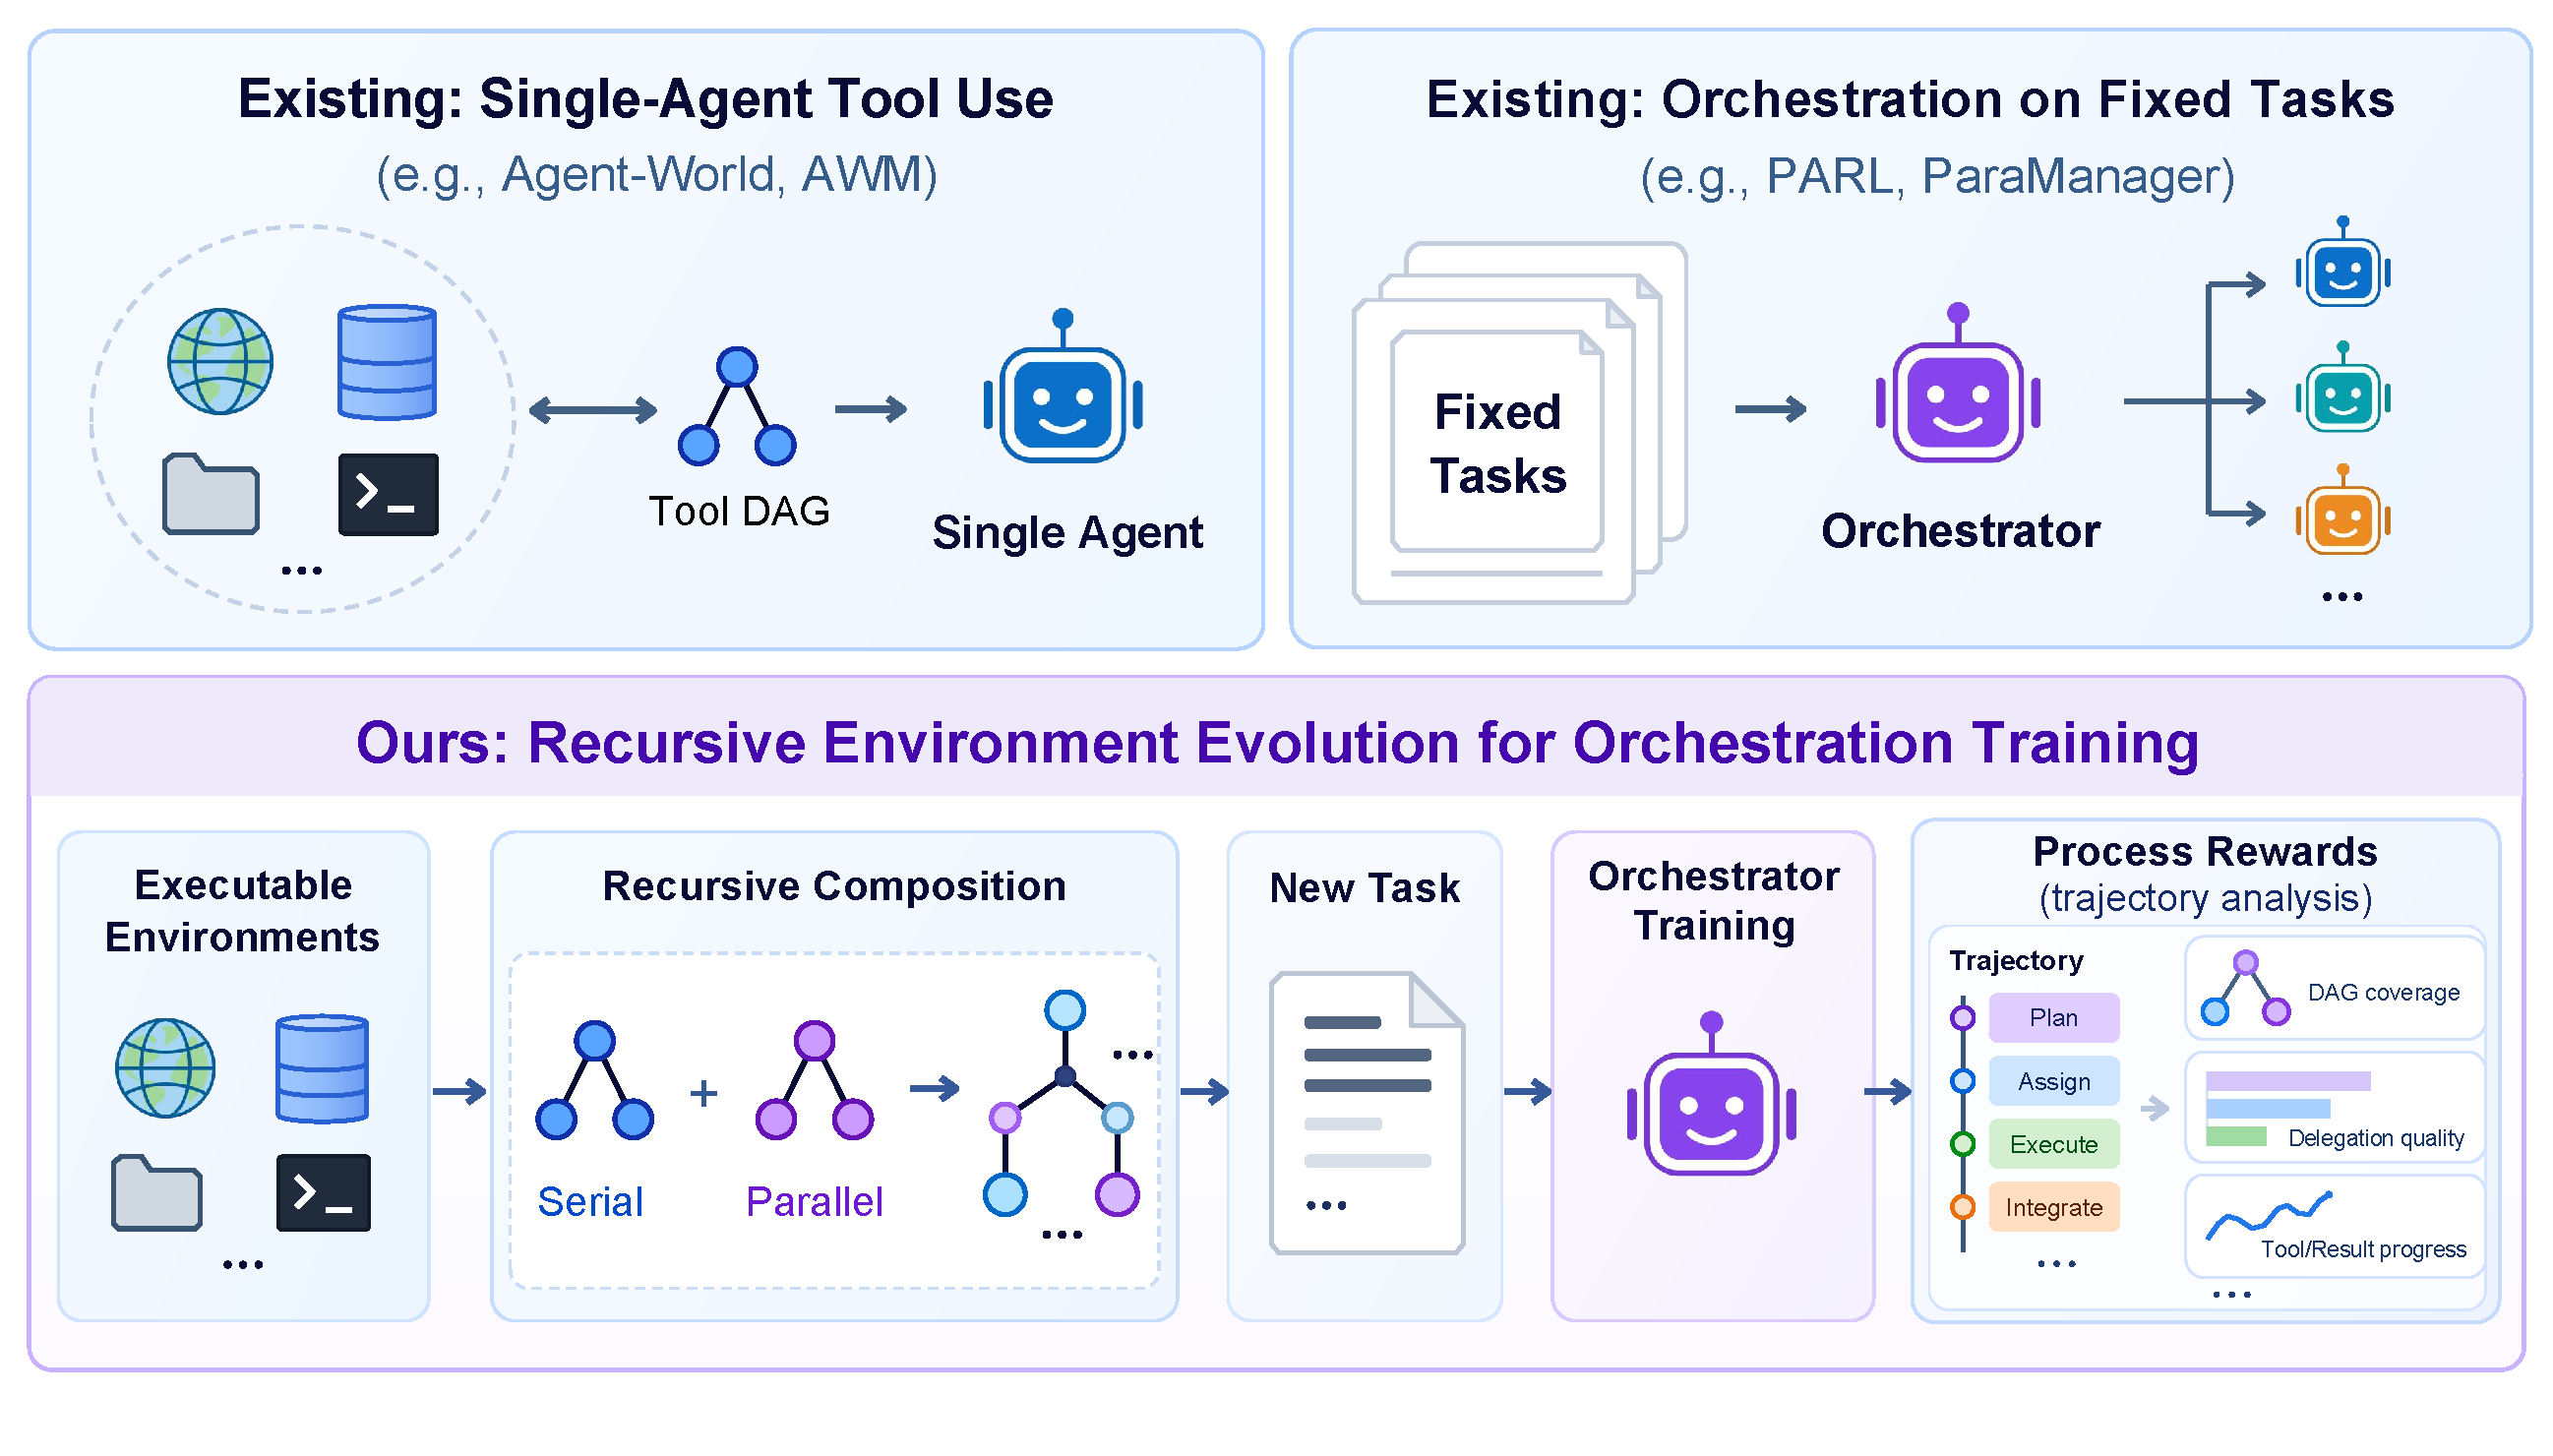
\includegraphics[width=0.97\linewidth]{figures/figure1.pdf}
  \caption{Existing environment synthesis builds executable tools and a verifier for one agent, and existing orchestration training consumes a fixed task set whose branch structure it does not control. MAW evolves the tasks of an executable environment by recursive environment improvement and trains an orchestrator on the resulting branches under schedule-aware process rewards.}
  \label{fig:teaser}
\end{figure}

To this end, we introduce \emph{Multi-Agent World} (MAW), an end-to-end framework for developing multi-agent orchestration.
As shown in Figure~\ref{fig:teaser}, MAW couples multi-agent environment synthesis with reinforcement learning inside the synthesized environments.
Specifically, to close the structural gap, MAW synthesizes multi-agent environments by \emph{recursive environment improvement}.
A serial operator links a subtask to the effect it consumes, and a parallel operator places independent subtasks on separate branches.
Applying the two operators recursively grows a reference task graph, which semantic reconstruction then rewrites into one coherent user request.
After the reference executes, replays from a fresh state, and passes semantic review, MAW admits the task into the training set.
To close the supervision gap, MAW trains the orchestrator with \emph{schedule-aware process rewards}.
These rewards read the recorded execution of the whole team and score tool progress, answer coverage, evidence delivery, and the quality of the schedule itself.
MAW connects the two mechanisms through one record.
Composition writes the branch structure into a task, and in the same step records which subtasks are verified as independent.
This record distinguishes a correct parallel decomposition from one that succeeds by chance.
Multi-agent environment synthesis therefore produces both the environment in which the team acts and the ground truth against which the orchestrator is rewarded.

We evaluate MAW on six agentic benchmarks covering multi-turn tool use, interactive task completion, executable multi-step tasks, long-horizon planning, broad information seeking, and real-world tool execution.
Experimental results show that MAW improves task success by \fillin\ over its single-agent initialization and by \fillin\ over the same multi-agent runtime without an orchestration update, while shortening the execution critical path by \fillin.
More importantly, the ablations show that the branches introduced by composition, and not the additional length of a composed task, account for the improvement.
Our contributions are three-fold.
\begin{itemize}[leftmargin=1em, itemsep=-1ex, topsep=0ex]
  \item \textbf{End-to-End Multi-Agent Framework}: To the best of our knowledge, MAW is the first framework that develops multi-agent orchestration end to end, synthesizing multi-agent environments and training the orchestrator inside them, where the construction record of a task also serves as the ground truth of its reward.
  \item \textbf{Recursive Environment Improvement and Schedule-Aware Rewards}: We propose recursive environment improvement, which converts single-agent environments into multi-agent environments by treating branch structure as a controlled construction variable, and schedule-aware process rewards, which make the quality of a decomposition visible in the gradient before any complete solution is sampled.
  \item \textbf{Strong Performance}: Experimental results on six agentic benchmarks show that MAW improves task success by \fillin\ with an 8B backbone, and behavior audits show that the gain comes from fewer duplicated assignments and fewer missing integrations.
\end{itemize}
